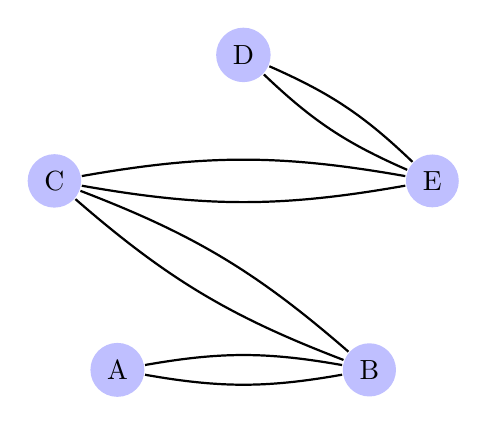
\begin{tikzpicture}
[thick,scale=.8,auto=left,every node/.style={circle,fill=blue!25}]
  \node (na) at (2,0) {A};
  \node (nb) at (6,0) {B};
  \node (nc) at (1,3) {C};
  \node (nd) at (4,5) {D};
  \node (ne) at (7,3) {E};

  \path[-,draw,thick,black,bend right=10]
  	(na) edge (nb)
  	(nc) edge (nb)
  	(nc) edge (ne)
  	(ne) edge (nd);
  
  \path[-,draw,thick,black,bend left=10]
  	(na) edge (nb)
  	(nc) edge (nb)
  	(nc) edge (ne)
  	(ne) edge (nd);
\end{tikzpicture}